\documentclass{beamer}
\usepackage{graphicx}
\usepackage{amsmath}
\usepackage{subfig}
\usepackage{listings}

% Set theme and colors
\usecolortheme{default}

% Set font family and other configurations
\usepackage{lmodern}
\renewcommand{\familydefault}{\sfdefault}
\setbeamertemplate{navigation symbols}{}


\title{Mixed Effects Models - Day 2}
\subtitle{Refreshing Linear Models I}
\author{Marieke Wesselkamp \\ Department of Biometry and Environmental Systems Analysis \\ Albert-Ludwigs-University of Freiburg (Germany)}
\date{February 2023}

\begin{document}

\begin{frame}
  \titlepage
\end{frame}

\begin{frame}{Recap Yesterday}
  \begin{itemize}
    \item Representative sampling vs. grouping of data
  \end{itemize}
  
  \begin{figure}[h]
    \centering
    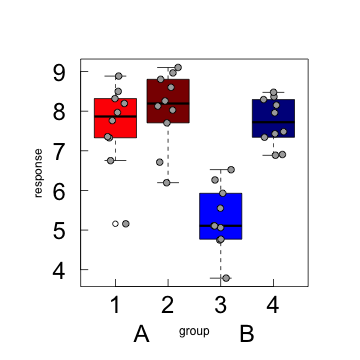
\includegraphics[width=0.5\textwidth]{lectures/day_2_LM_refresh_I/figures/unnamed-chunk-3-1.png}
    \caption{Boxplot showing response by group.}
  \end{figure}
\end{frame}

\begin{frame}{The Statistical Model}
  \begin{quote}
    In science, we want to make general statements about the world from limited, messy data. Statistical models help us do that.
  \end{quote}
  
  \begin{itemize}
    \item A \textbf{statistical model} is an idealized description of how the data were generated, by which processes the data came to be realized, and the relationships between factors.
    \item A good model separates the deterministic signal from the stochastic noise.
  \end{itemize}
\end{frame}

\begin{frame}
  \frametitle{Model Example}
  \begin{block}{}
    This (fictitious) relationship between nutrient concentration and plant biomass...
  \end{block}
  
  \begin{figure}[h]
    \centering
    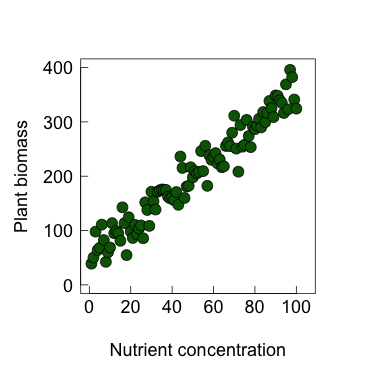
\includegraphics[width=0.45\textwidth]{lectures/day_2_LM_refresh_I/figures/unnamed-chunk-4-1.png}
    \caption{Scatterplot of nutrient concentration vs. plant biomass.}
  \end{figure}
    \tiny{(Can you spot why this example is likely nonsense from a biological perspective? Think about what happens at a nutrient concentration of 0)}
\end{frame}

\begin{frame}
  \frametitle{Linear Model}
  \begin{block}{}
    ...can be described by this \textbf{model}:
  \end{block}

  \begin{equation}
  y = \beta_0 + \beta_1 \cdot x + \epsilon
  \end{equation}

  \begin{figure}[h]
    \centering
    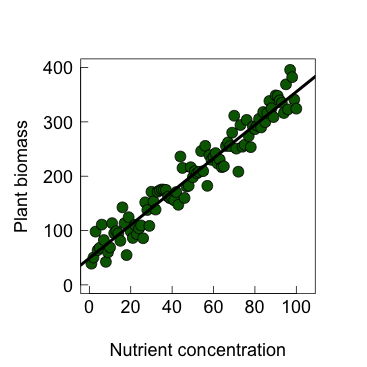
\includegraphics[width=0.5\textwidth]{lectures/day_2_LM_refresh_I/figures/unnamed-chunk-5-1.png} 
    \caption{Linear model fit to the data.}
  \end{figure}
\end{frame}

\begin{frame}
  \frametitle{Deterministic Part}
  \begin{itemize}
    \item The \textbf{deterministic} part $y = \beta_0 + \beta_1 \cdot x$ describes how one thinks this little part of the world works, with $\beta_0$ and $\beta_1$ as the \textbf{model parameters}\footnote{\small Intercept and slope in this case}
  \end{itemize}
  
  \begin{figure}[h]
    \centering
    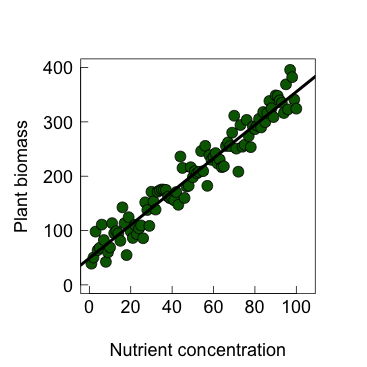
\includegraphics[width=0.5\textwidth]{lectures/day_2_LM_refresh_I/figures/unnamed-chunk-6-1.png} 
    \caption{Deterministic model for nutrient concentration vs. plant biomass.}
  \end{figure}
\end{frame}

\begin{frame}
  \frametitle{Incorrect Deterministic Model}
  \begin{itemize}
    \item Getting the deterministic part right is crucial for meaningful statistical modeling.
    \item \small Obviously, this is the wrong deterministic model for the observed data: the intercept is too high and the slope too shallow.
  \end{itemize}
  
  \begin{figure}[h]
    \centering
    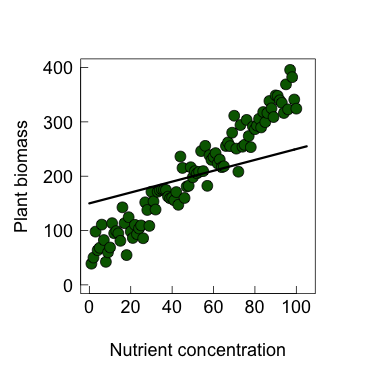
\includegraphics[width=0.5\textwidth]{lectures/day_2_LM_refresh_I/figures/unnamed-chunk-7-1.png} 
    \caption{Incorrect deterministic model.}
  \end{figure}
\end{frame}

\begin{frame}
  \frametitle{Another Incorrect Model}
  \begin{block}{}
    And this deterministic part $y = \frac{a \cdot x}{1 + a \cdot h \cdot x}$ would be wrong, too!
  \end{block}
  
  \begin{figure}[h]
    \centering
    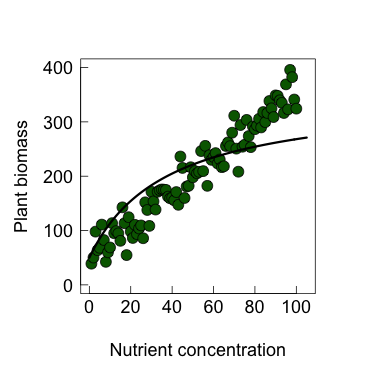
\includegraphics[width=0.5\textwidth]{lectures/day_2_LM_refresh_I/figures/unnamed-chunk-8-1.png} 
    \caption{Another incorrect deterministic model.}
  \end{figure}
\end{frame}

\begin{frame}
  \frametitle{The Stochastic Part}
      The \textbf{stochastic} part $\epsilon$ describes how values scatter around the deterministic model. \small Such scatter can come from errors during measurements and from factors or covariates not included in the deterministic part. It is, however, often a characteristic of the underlying data generation process.
  
  \begin{figure}[h]
    \centering
    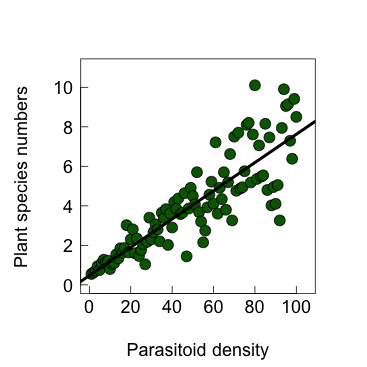
\includegraphics[width=0.5\textwidth]{lectures/day_2_LM_refresh_I/figures/unnamed-chunk-9-1.png} 
    \caption{Stochastic part of the model.}
  \end{figure}
\end{frame}

\begin{frame}
    \frametitle{}
    \textbf{Two different stochastic processes generate different forms of scatter around the deterministic core.}
    
    \begin{figure}[h]
        \centering
        \subfloat[Poisson]{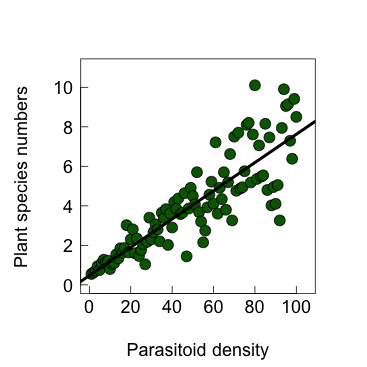
\includegraphics[width=0.5\textwidth]{lectures/day_2_LM_refresh_I/figures/unnamed-chunk-10-1.png}\label{a) Poisson process}}
        \subfloat[Gaussian]{{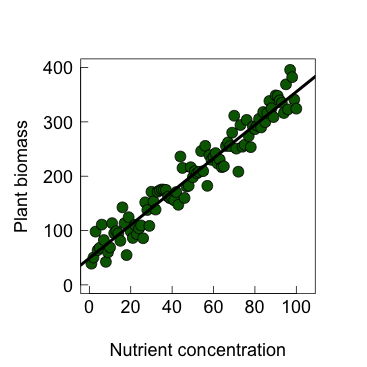
\includegraphics[width=0.5\textwidth]{lectures/day_2_LM_refresh_I/figures/unnamed-chunk-11-1.png}\label{b) Gaussian process}}} 
    \end{figure}
\end{frame}

\begin{frame}
    \frametitle{Gaussian Process in Linear Models}
    In Linear Models, a Gaussian process is assumed to govern the stochastic part of the model. The full assumptions regarding the stochastic part amount to:
    \begin{equation*}
        \epsilon \text{ is \textit{iid}}, \quad \epsilon \sim \mathcal{N}(0, \sigma^2_{\epsilon})
    \end{equation*}
    \begin{itemize}
        \item $\epsilon$ is \textit{iid} stands for \textit{independently and identically distributed}, meaning each error is uncorrelated with the others and the error distribution around the deterministic trend is identical at each value of the predictor. \footnote{\textbf{Note:} This is clearly not the case in the left figure on the previous slide. There, the distribution is much wider for high values of parasitoid density—a typical feature of count data.} 
        \item $\epsilon \sim \mathcal{N}(0, \sigma^2_{\epsilon})$ indicates that the errors are assumed to be normally distributed with a mean of 0 and variance of $\sigma^2$. 
    \end{itemize}
\end{frame}

\begin{frame}
    \frametitle{}
    $y = \beta_0 + \beta_1 \cdot x + \epsilon$, $\epsilon_{iid} \sim \mathcal{N}(0, \sigma^2_{\epsilon})$ \\
    \vspace{0.5cm}
    \textbf{The four assumptions of the Linear Model:}
    \begin{itemize}
        \item \textbf{Normality:} $y$ is normally distributed at any value of $x$, implying residuals are normally distributed.
        \item \textbf{Homogeneity:} The variance of the residuals is the same at any value of $x$.
        \item \textbf{Independence:} Measurements are independent of each other.
        \item \textbf{Linearity:} The relationship between $y$ and $x$ is linear and $x$ is deterministic.
    \end{itemize}
    
\end{frame}

\begin{frame}
    \frametitle{}
    \begin{center}
        \huge\textbf{\textcolor{purple}{The linear model in matrix notation}}
    \end{center}
\end{frame}

\begin{frame}
    \frametitle{}
    \begin{equation*}
        y = \beta_0 + \beta_1 \cdot x + \epsilon, \quad \epsilon_{iid} \sim \mathcal{N}(0, \sigma^2_{\epsilon})
    \end{equation*}
    \text{can also be written as}
    \begin{equation*}
        \mathbf{y} = \mathbf{X} \cdot \mathbf{b} + \mathbf{e}, \quad \epsilon \sim \mathcal{N}(0, \sigma^2_{\epsilon} \cdot \mathbf{I})
    \end{equation*}
    where $\mathbf{y}$ are the measured response values, $\mathbf{X}$ is the Design matrix, $\mathbf{b}$ is a vector of the model parameters, $\mathbf{e}$ is a vector of the errors, and $\sigma^2_{\epsilon} \cdot \mathbf{I}$ is the variance-covariance matrix of the errors, obtained by multiplying the estimated residual variance $\sigma^2_{\epsilon}$ with an identity matrix. \footnote{\textbf{Note:} Throughout, symbols for matrices will be in bold.}
    

\end{frame}

\begin{frame}
    \frametitle{Let's Break This Down}
    Imagine we have $n = 5$ measured values $y_i$ with $i = 1, \ldots, n$, we get the response vector:
    \vspace{0.5cm}
    \begin{equation*}
        \mathbf{y} = \left( \begin{array}{c} y_1 \\ y_2 \\ y_3 \\ y_4 \\ y_5 \end{array}\right) = \left( \begin{array}{c} 2.03 \\ 4.31 \\ 7.12 \\ 6.62 \\ 11.07 \end{array}\right) 
    \end{equation*}    
\end{frame}

\begin{frame}
    \frametitle{}
    \textbf{The design matrix encodes the design of the experiments. The first column has all 1's for the intercept, and the second column contains the $y_i$ values of the continuous predictor:}
    \begin{equation*}
        \mathbf{x} = \left( \begin{array}{cc} 1 & x_1 \\ 1 & x_2 \\ 1 & x_3 \\ 1 & x_4 \\ 1 & x_5 \end{array}\right) = \left( \begin{array}{cc} 1 & 1.27 \\ 1 & 1.47 \\ 1 & 2.47 \\ 1 & 2.94 \\ 1 & 3.61 \end{array}\right)
    \end{equation*}
\end{frame}

\begin{frame}
    \frametitle{}
    We have the deterministic model $y = \beta_0 + \beta_1 \cdot x$, i.e., there are two parameters, giving the parameter vector:
    \begin{equation*}
        \mathbf{b} = \left( \begin{array}{c} \beta_0 \\ \beta_1 \end{array}\right) = \left( \begin{array}{c} \text{intercept} \\ \text{slope} \end{array}\right) = \left( \begin{array}{c} -1.44 \\ 3.27 \end{array}\right)
    \end{equation*}
\end{frame}

\begin{frame}
    \frametitle{}
    Finally, the stochastic part $\epsilon$, i.e., $i$ deviations $\epsilon_i$ with $i = 1, \ldots, n$ from the $n = 5$ measured $y_i$:
    \begin{equation*}
        \mathbf{e} = \left( \begin{array}{c} \epsilon_1 \\ \epsilon_2 \\ \epsilon_3 \\ \epsilon_4 \\ \epsilon_5 \end{array}\right) = \left( \begin{array}{c} -0.69 \\ 0.95 \\ 0.53 \\ -1.53 \\ 0.74 \end{array}\right)
    \end{equation*}
\end{frame}

\begin{frame}
    \frametitle{}
    With $\epsilon_{iid} \sim \mathcal{N}(0, \sigma^2_{\epsilon})$, given in matrix notation by:
    \begin{equation*}
        \scriptsize{\sigma^2 \cdot \mathbf{I} = 1.52 \cdot \left( \begin{array}{ccccc} 1 & 0 & 0 & 0 & 0 \\ 0 & 1 & 0 & 0 & 0 \\ 0 & 0 & 1 & 0 & 0 \\ 0 & 0 & 0 & 1 & 0 \\ 0 & 0 & 0 & 0 & 1 \end{array}\right)}
    \end{equation*}
    \begin{equation*}
        \scriptsize{= \left( \begin{array}{ccccc} 1.52 & 0 & 0 & 0 & 0 \\ 0 & 1.52 & 0 & 0 & 0 \\ 0 & 0 & 1.52 & 0 & 0 \\ 0 & 0 & 0 & 1.52 & 0 \\ 0 & 0 & 0 & 0 & 1.52 \end{array}\right)}
    \end{equation*}
\end{frame}

\begin{frame}
    \frametitle{}
    \textbf{Why all this math?}
    
    The point is that the last matrix, the variance-covariance matrix of the errors, actually encodes, among other things, the assumption of independence.

    In row $i$ and column $j$, you find the covariances $d_{ij}$ of an $error_i$ with an $error_j$. As long as these \textbf{off-diagonal} values are 0, the assumption of data points' independence is fulfilled.
\end{frame}

\begin{frame}
    \frametitle{}
    \begin{equation*}
        \scriptsize{\sigma^2 \cdot \mathbf{I} = \left( \begin{array}{ccccc} 1.52 & 0 & 0 & 0 & 0 \\ 0 & 1.52 & 0 & 0 & 0 \\ 0 & 0 & 1.52 & 0 & 0 \\ 0 & 0 & 0 & 1.52 & 0 \\ 0 & 0 & 0 & 0 & 1.52 \end{array}\right)}
    \end{equation*}
    
    \vspace{1cm}
    \textbf{\textcolor{purple}{Mixed Effects Models allow the covariances $d_{ij}$ in the off-diagonals to be non-zero.}}
\end{frame}

\begin{frame}
    \frametitle{}
    \begin{center}
        \huge\textbf{\textcolor{purple}{Parameter and variance estimation in linear models}}
    \end{center}
\end{frame}

\begin{frame}
    \frametitle{How do we get the values for the betas and sigma?}
    The $y_i$s are measured, and the $x_i$s are given. What is now wanted are the $\beta$s and $\sigma^2$. Two common estimation approaches:
    \begin{enumerate}
        \item \textbf{(Ordinary) least squares}
        \item \textbf{Maximum Likelihood estimation (ML)}
    \end{enumerate}
\end{frame}

\begin{frame}
    \frametitle{Ordinary Least Squares}
    We get an estimation for the unknown regression parameters $\beta$ by minimizing the sum of squares:
    \begin{equation*}
        OLS(\beta) = \sum_{i=1}^{n} (y_i - \mathbf{x}'_i \mathbf{\beta})^2 = (\mathbf{y} - \mathbf{X \beta})'(\mathbf{y} - \mathbf{X \beta})
    \end{equation*}
    \vspace{0.5cm}
    
    This minimization problem has a unique solution for $\mathbf{\hat{\beta}}$, given the columns of $\mathbf{X}$ are linearly independent:
    \begin{equation*}
        \mathbf{\hat{\beta}} = (\mathbf{X}'\mathbf{X})^{-1} \mathbf{X}'\mathbf{Y}
    \end{equation*}
\end{frame}

\begin{frame}
    \frametitle{}
    After estimation of $\mathbf{\hat{\beta}}$, we get an estimate for the variance $\sigma^2$:
    \begin{equation*}
        \hat{\sigma}^2 = \frac{(\mathbf{y} - \mathbf{X} \mathbf{\hat{\beta}})' (\mathbf{y} - \mathbf{X} \mathbf{\hat{\beta}})}{n-p-1} = \frac{(\mathbf{y} - \hat{\mathbf{y}})' (\mathbf{y} - \hat{\mathbf{y}})}{n-p-1}
    \end{equation*}
\end{frame}

\begin{frame}{In R}
    \scalebox{0.75}{
      \lstinputlisting[]{lectures/day_2_LM_refresh_I/outputs/output_1.txt}
      }
\end{frame}

\begin{frame}{In R}
    \scalebox{0.7}{
      \lstinputlisting[]{lectures/day_2_LM_refresh_I/outputs/output_2.txt}
      }    
\end{frame}

\begin{frame}
    \frametitle{Maximum Likelihood Estimation}
    The OLS estimator for $\mathbf{{\beta}}$ is received without any assumption on the stochastic parts of the model.
    
    ML estimation is based on an assumption about the data-generating distribution, i.e., in the case of the linear model, the normal distribution (\textit{Normality}).
    
    The likelihood $L$ tells us how plausible our observations are, given a set of parameters:
    \begin{equation*}
        L(y | \theta), \quad \text{with} \quad y \sim N(\mu, \sigma^2)
    \end{equation*}
\end{frame}

\begin{frame}
    \frametitle{}
    Assuming a normal error distribution, this is:
    \begin{equation*}
        \scriptsize{L( y | \beta, \sigma^2) = L(y_i|\mu = \beta_0 + \beta_1 \cdot x_i, \sigma^2) = \prod_{i=1}^n \frac{1}{\sigma \sqrt{2 \pi}} e^\frac{-(y_i - (\mu = \beta_0 + \beta_1 \cdot x_i))^2}{2 \sigma}}
    \end{equation*}
    \vspace{0.5cm}
    
    Because taking the product of $L$ gives ultimately very small numbers, this expression is transformed to the \textbf{Log-Likelihood} $LL$:
    \begin{multline*}
        LL(y_i | \mu = \beta_0 + \beta_1 x_i, \sigma) = \\
        -n \ln \sigma^2 - \frac n2 \ln (2 \pi) - \frac{1}{2 \sigma^2} \sum (y_i - (\mu = \beta_0 + \beta_1 x_i))^2    
    \end{multline*}
    which is then maximized by differentiation.
\end{frame}

\begin{frame}
    \frametitle{}
    \textbf{There are analytical solutions only for a few problems (like ours). In these cases, however, the MLE can be calculated in three steps:}
    \begin{enumerate}
        \item Find the (partial) derivative of $LL$ for each parameter.
        \item Set it to zero (a function has its maximum where its first derivative is zero).
        \item Solve the derivative for the parameter.
        \item Verify the maximum with the second derivative.
    \end{enumerate}
\end{frame}

\begin{frame}
    \frametitle{}
    \textbf{The steeper $LL$ around its maximum, the more negative its second derivative, and the smaller the standard errors.}
    
    \begin{figure}[h]
        \centering
        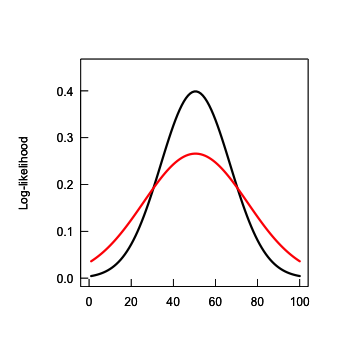
\includegraphics[width=0.5\textwidth]{lectures/day_2_LM_refresh_I/figures/unnamed-chunk-19-1.png} 
        \caption{Log-likelihood plot}
    \end{figure}
\end{frame}

\begin{frame}
    \frametitle{}
    \begin{center}
        \huge\textbf{\textcolor{purple}{Break!}}
    \end{center}
\end{frame}

\begin{frame}
    \frametitle{The Parameter Variance-Covariance Matrix}
    The parameter variance-covariance matrix tells how the estimated parameters are correlated. It is obtained from the \textbf{second} derivative of the log-likelihood function $\ell$.

    \vspace{0.5cm}
    Standard errors tell how precisely a parameter has been estimated. They are calculated by taking the square root of the diagonal values in the parameter variance-covariance matrix:
    \begin{equation*}
        \scriptsize{cov(\mathbf{\hat{\beta}})=\sigma^2 (\mathbf{X}' \mathbf{X})^{-1}}
    \end{equation*}
\end{frame}

\begin{frame}{In R this can be done as}
    \scalebox{0.8}{
      \lstinputlisting[]{lectures/day_2_LM_refresh_I/outputs/output_3.txt}
      }    
\end{frame}

\begin{frame}
    \frametitle{Optimisation Techniques}
    \textbf{For most problems, an analytical solution does not exist because derivatives cannot be found or solved. $\mathbf{\hat{\beta}}$ and $\sigma^2$ are then estimated using an iterative ML \color{blue}{optimisation procedure}.}
\end{frame}

\begin{frame}
    \frametitle{Example: Grid Search}
    Our $n = 5$ response values $y_i$ measured at predictor values $x_i$ with $i = 1,...,n$
    
    \begin{figure}[h]
        \centering
        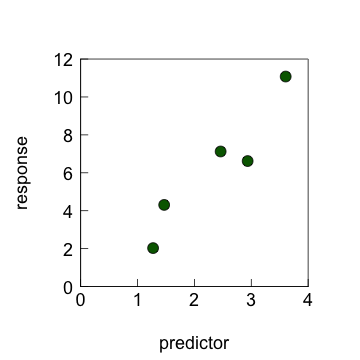
\includegraphics[width=0.5\textwidth]{lectures/day_2_LM_refresh_I/figures/unnamed-chunk-22-1.png} 
        \caption{Grid search example}
    \end{figure}
\end{frame}

\begin{frame}
    \frametitle{}
    Compute the log-likelihood for a random initialization of $\beta_0$ and $\beta_1$, with $\beta_0 = -5$ and $\beta_1 = 5$:
    
    \vspace{0.5cm}
    
    \begin{columns}
        \begin{column}{0.5\textwidth}
            \begin{multline*}
            -5 \ln \sigma - \frac 52 \ln (2 \pi) \\
            - \frac{1}{2 \sigma^2} [( 2.03 - (-5 + 5 \cdot 1.27))^2 \\
            + ( 4.31 - (-5 + 5 \cdot 1.47))^2 \\
            + ( 7.12 - (-5 + 5 \cdot 2.46))^2 \\
            + ( 6.62 - (-5 + 5 \cdot 2.94))^2 \\
            + ( 11.08 - (-5 + 5 \cdot 3.61))^2] \\
            \textbf{= 0.80}
            \end{multline*}  
        \end{column}
        
        \begin{column}{0.5\textwidth}
            \centering
            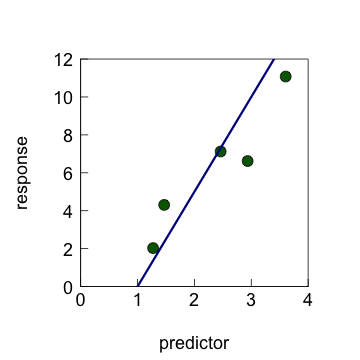
\includegraphics[width=\textwidth]{lectures/day_2_LM_refresh_I/figures/unnamed-chunk-23-1.png}
        \end{column}
    \end{columns}
\end{frame}

\begin{frame}
    \frametitle{}
    But $\beta_0 = -1.44$ and $\beta_1 = 3.27$ give:
    
    \vspace{0.5cm}
    
    \begin{columns}
        \begin{column}{0.5\textwidth}
            \begin{multline*}
            -5 \ln \sigma - \frac 52 \ln (2 \pi) \\
            - \frac{1}{2 \sigma^2} [( 2.03 - (-1.44 + 3.27 \cdot 1.27))^2 \\
            + ( 4.31 - (-1.44 + 3.27 \cdot 1.47))^2 \\
            + ( 7.12 - (-1.44 + 3.27 \cdot 2.46))^2 \\
            + ( 6.62 - (-1.44 + 3.27 \cdot 2.94))^2 \\
            + ( 11.08 - (-1.44 + 3.27 \cdot 3.61))^2] \\
            \textbf{= 1.23 = maximal Log-Likelihood $\ell$}
            \end{multline*}  
        \end{column}
        
        \begin{column}{0.5\textwidth}
            \centering
            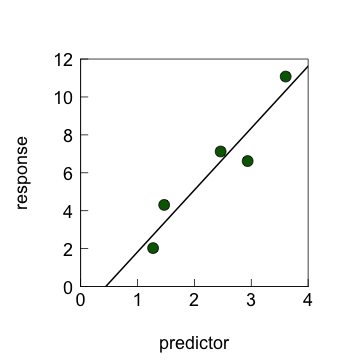
\includegraphics[width=\textwidth]{lectures/day_2_LM_refresh_I/figures/unnamed-chunk-24-1.png}
        \end{column}
    \end{columns}
\end{frame}

\begin{frame}
    \frametitle{}
    \begin{columns}
        \begin{column}{0.5\textwidth}
            In a grid search, the Likelihood is systematically calculated across combined ranges of $\beta_0$ and $\beta_1$ in order to find the best values, i.e., find the MLEs for them:
        \begin{multiline*}
        \beta_0 = -1.44\\
        \beta_1 = 3.27\\
        \end{multiline*}
        \end{column}
        \begin{column}{0.5\textwidth}
            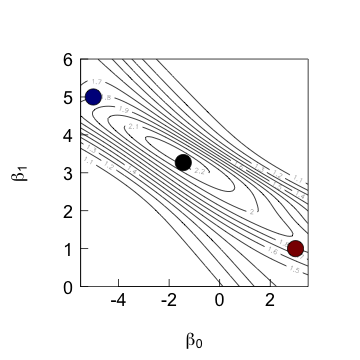
\includegraphics[width=\textwidth]{lectures/day_2_LM_refresh_I/figures/unnamed-chunk-25-1.png}
        \end{column}
    \end{columns}
\end{frame}

\begin{frame}
    \frametitle{}
    \textbf{In Mixed Effects Models, other optimisation procedures are used to get parameters and standard errors, which are derivative-based or derivative-free algorithms.}\\
    \vspace{0.5cm}
    Example: Quasi-Newton method (method = c("BFGS")):
    \vspace{0.5cm}
    \scalebox{0.7}{
      \lstinputlisting[]{lectures/day_2_LM_refresh_I/outputs/output_4.txt}
    }    
\end{frame}

\begin{frame}
    \frametitle{}
    \textbf{With only five data points, optimisers work rather poorly:}
    
    Remember the optimal values for $\beta_0 = -1.44$ and $\beta_1 = 3.27$ that we calculated analytically.
    \vspace{0.5cm}
    
    \scalebox{0.7}{
      \lstinputlisting[]{lectures/day_2_LM_refresh_I/outputs/output_5_1.txt}
    }
    \vspace{0.5cm}
    
    To compute standard errors of the estimates, extract the second derivatives from the hessian matrix.
    \vspace{0.5cm}
    
    \scalebox{0.7}{
      \lstinputlisting[]{lectures/day_2_LM_refresh_I/outputs/output_5_2.txt}
    }
    \vspace{0.5cm}
    
    \tiny{\url{https://stats.stackexchange.com/questions/68080/basic-question-about-fisher-information-matrix-and-relationship-to-hessian-and-s?rq=1}}
    
\end{frame}

\begin{frame}
    \frametitle{}
    \begin{center}
        \huge\textbf{\textcolor{purple}{Predictions with a linear model}}
    \end{center}
\end{frame}

\begin{frame}
    \frametitle{}
    \begin{columns}
        \begin{column}{0.5\textwidth}
            \textbf{Once we have obtained the MLE estimates, one can use the model to make predictions.}
            \vspace{0.5cm}
    
            Just plug into the equation $y = \beta_0 + \beta_1 \cdot x$ the predictor values you wish to obtain so far not measured response values for:
            \vspace{0.5cm}
            
            For example, the new data point for $x = 2$ is $y = -1.440 + 3.266 \cdot 2 = 5.1$.
        \end{column}
        \begin{column}{0.5\textwidth}
            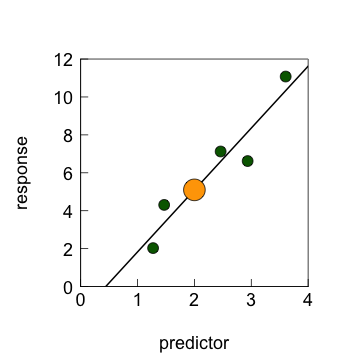
\includegraphics[width=\textwidth]{lectures/day_2_LM_refresh_I/figures/unnamed-chunk-29-1.png}    
        \end{column}
    \end{columns}
\end{frame}

\begin{frame}
    \frametitle{Predictions in Matrix Notation}
    \begin{equation*}
        \hat{y} = \mathbf{X \hat{\beta}}
    \end{equation*}
    In R:
    \vspace{0.5cm}
    
    1) New data to the new design matrix X
    \scalebox{0.65}{
      \lstinputlisting[]{lectures/day_2_LM_refresh_I/outputs/output_6_1.txt}
    }
    \vspace{0.5cm}
    
    2) Matrix-multiply X by the parameter vector $\hat\beta$ to get the predictions
    
    \scalebox{0.65}{
      \lstinputlisting[]{lectures/day_2_LM_refresh_I/outputs/output_6_2.txt}
    }
\end{frame}

\begin{frame}
    \frametitle{Estimate the Standard Errors}
    Estimate the standard errors using the parameter variance-covariance matrix:
    \begin{equation*}
        \mathbf{V} = cov(\mathbf{\hat{\beta}})=\sigma^2 (\mathbf{X}' \mathbf{X})^{-1}
    \end{equation*}
    In R:
    \vspace{0.5cm}

    3) Compute first the variance-covariance matrix \textbf{V} and then the prediction variances \textbf{XVX'} with the new design matrix

    \scalebox{0.65}{
      \lstinputlisting[]{lectures/day_2_LM_refresh_I/outputs/output_7_1.txt}
    }
    \vspace{0.5cm}
    
    4) Extract the diagonal of this matrix and take the square root. If computing prediction rather than confidence intervals, add the residual variance $\sigma^2$.

    \scalebox{0.7}{
      \lstinputlisting[]{lectures/day_2_LM_refresh_I/outputs/output_7_2.txt}
    }

    
\end{frame}

\begin{frame}
    \frametitle{}
    \begin{columns}
        \begin{column}{0.5\textwidth}
        5) Compute the 95\% confidence intervals based on a Normal approximation: $SE \cdot 1.96$   
        \scalebox{0.7}{
            \lstinputlisting[]{lectures/day_2_LM_refresh_I/outputs/output_8.txt}
        }
        \end{column}
        \begin{column}{0.5\textwidth}
        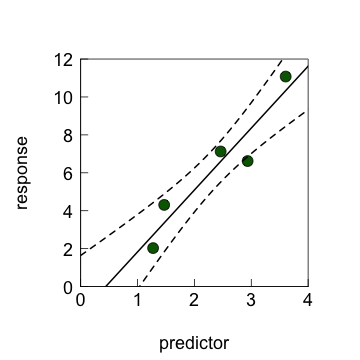
\includegraphics[width=\textwidth]{lectures/day_2_LM_refresh_I/figures/unnamed-chunk-35-1.png}    
        \end{column}
    \end{columns}


    
    
\end{frame}

\begin{frame}
    \frametitle{}
    \textbf{All that is built in R for Linear Models:}
    
    Fit model with Maximum Likelihood, extract ML estimates, and more.

    \scalebox{0.6}{
        \lstinputlisting[]{lectures/day_2_LM_refresh_I/outputs/output_9.txt}
    }
    
\end{frame}

\begin{frame}
    \centering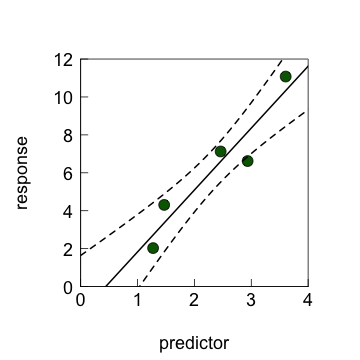
\includegraphics[width=0.6\textwidth]{lectures/day_2_LM_refresh_I/figures/unnamed-chunk-35-1.png}            
        
    \scalebox{0.7}{
        \lstinputlisting[]{lectures/day_2_LM_refresh_I/outputs/output_10.txt}
    }    
    
\end{frame}

\begin{frame}
    \frametitle{}
    \begin{center}
        \huge\textbf{\textcolor{purple}{Model validation: check your assumptions}}
    \end{center}
\end{frame}

\begin{frame}
    \frametitle{}
    \textbf{Before we trust the model output, we have to check whether the model assumptions are met.}

    \begin{columns}
        \begin{column}{0.5\textwidth}
        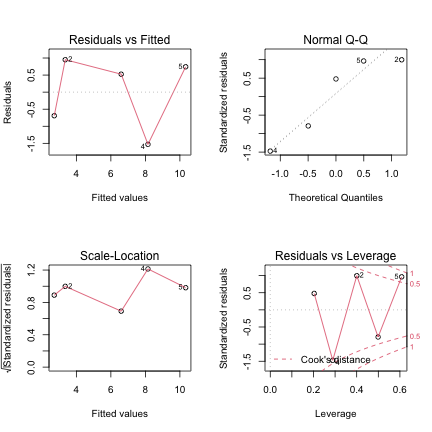
\includegraphics[width=\textwidth]{lectures/day_2_LM_refresh_I/figures/unnamed-chunk-40-1.png}     
        \end{column}
        \begin{column}{0.5\textwidth}
        \scalebox{0.7}{
            \lstinputlisting[]{lectures/day_2_LM_refresh_I/outputs/output_11.txt}
        }     
        \end{column}
    \end{columns}

\end{frame}

\begin{frame}
    \frametitle{The Idea of a Sick Model}
    \begin{figure}
        \centering
        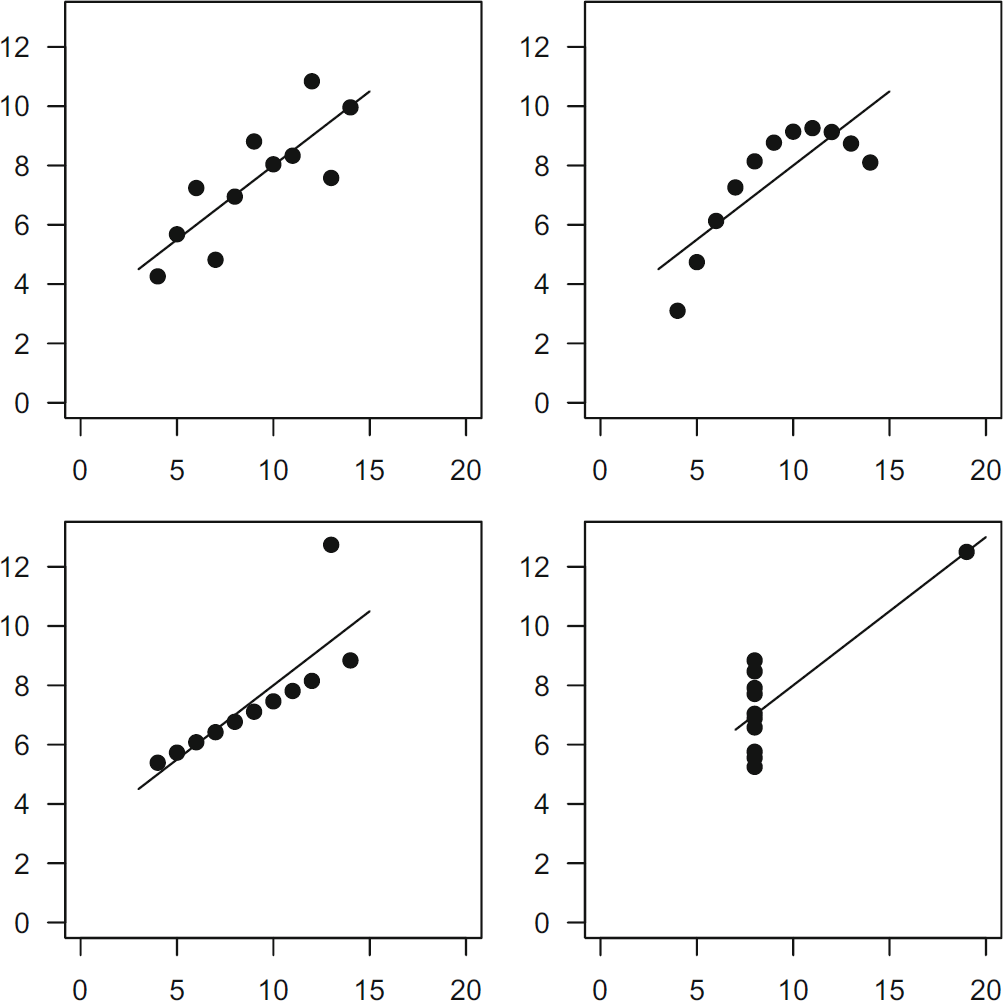
\includegraphics[width=0.6\textwidth]{lectures/day_2_LM_refresh_I/figures/Anscombe.png}
    \end{figure}
\end{frame}

\begin{frame}
    \frametitle{It's All About Residuals}
    \textbf{Difference between measured data and predicted values}
    
    \begin{figure}[h]
        \centering
        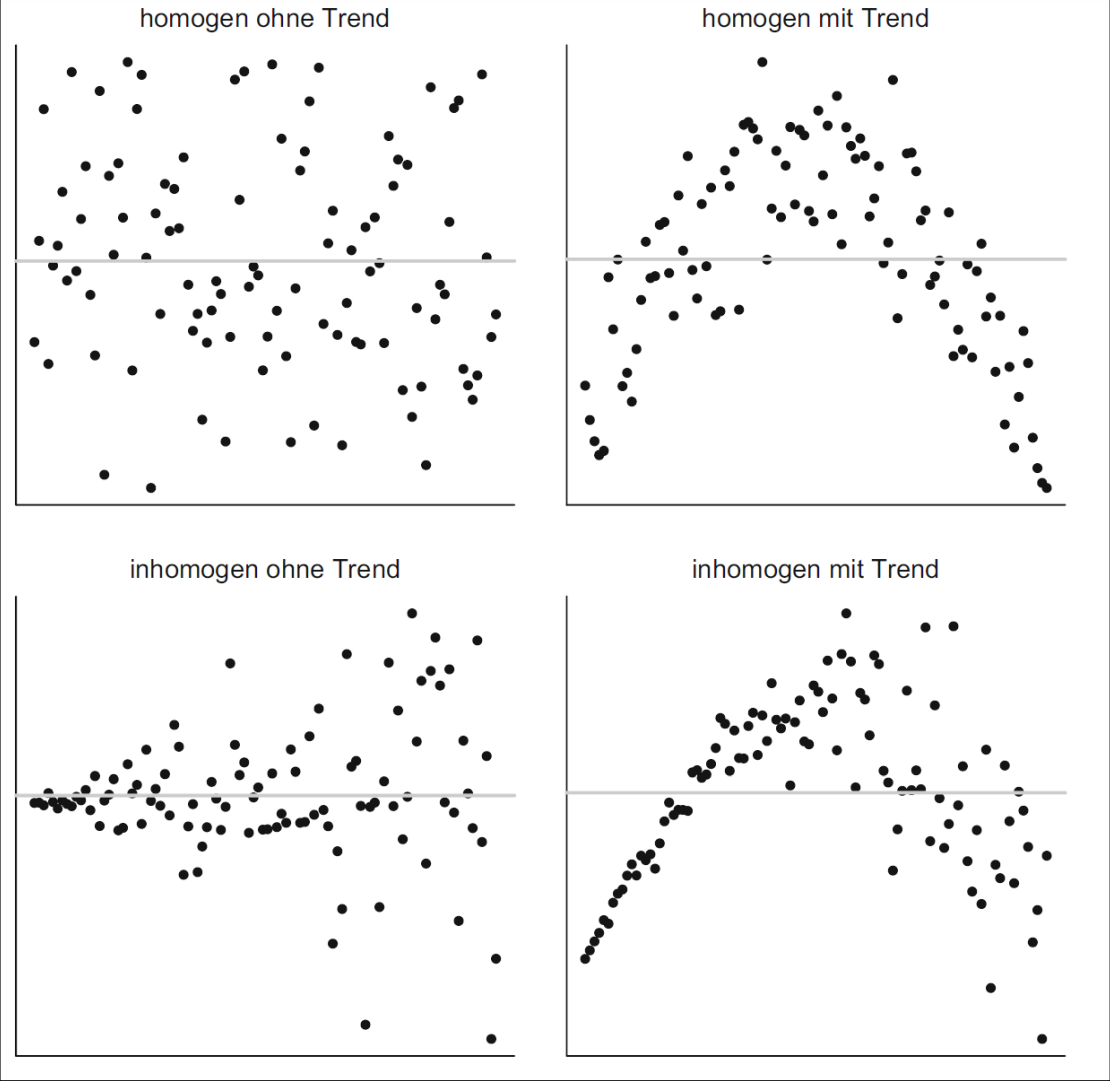
\includegraphics[width=0.5\textwidth]{lectures/day_2_LM_refresh_I/figures/residuals.png} 
    \end{figure}
\end{frame}

\begin{frame}
    \frametitle{Residual-Checks}

    \begin{columns}
        \begin{column}{0.5\textwidth}
        Trends? Misspecified deterministic part. Heteroscedasticity? Misspecified stochastic part (the errors) or missing information.    
        \end{column}
        \begin{column}{0.5\textwidth}
            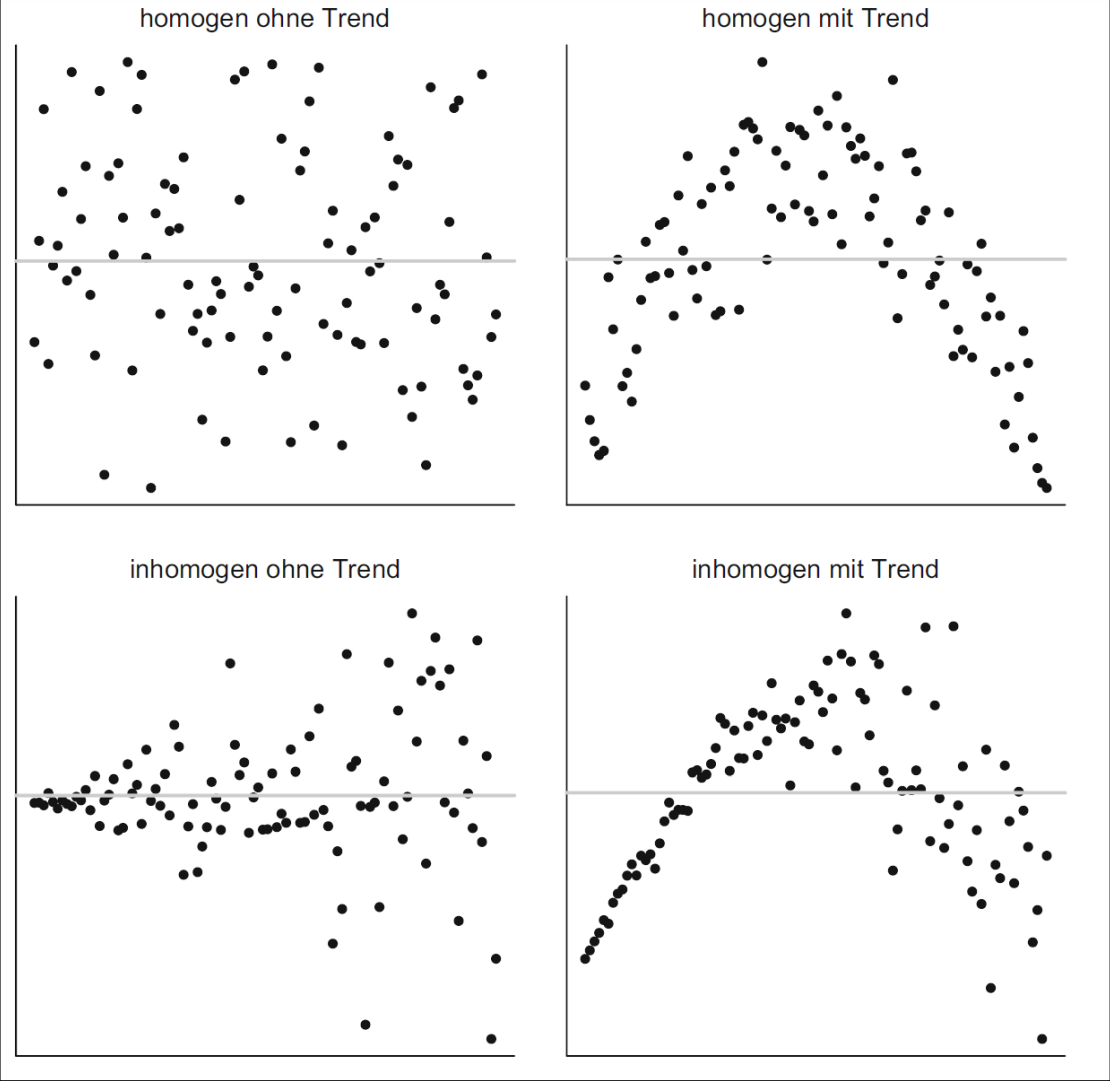
\includegraphics[width=\textwidth]{lectures/day_2_LM_refresh_I/figures/residuals.png}    
        \end{column}
    \end{columns}

\end{frame}

\begin{frame}
    \frametitle{The Fab Four}
        \centering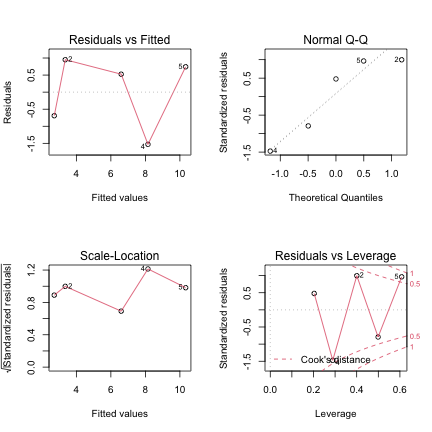
\includegraphics[width=0.7\textwidth]{lectures/day_2_LM_refresh_I/figures/unnamed-chunk-40-1.png} 
        \centering\scalebox{0.75}{
            \lstinputlisting[]{lectures/day_2_LM_refresh_I/outputs/output_12.txt}
        }
\end{frame}

\begin{frame}
    \large\textbf{How to interpret plot diagnostics for an lm object:}
    \url{https://stats.stackexchange.com/questions/58141/interpreting-plot-lm/65864}
\end{frame}

\begin{frame}
    \frametitle{}
    \textbf{WARNING:} Violations of the assumption of independence of data points cannot reliably be diagnosed. One simply has to know that from the study design!
\end{frame}

\begin{frame}
    \frametitle{}
    \textbf{Remember the example from yesterday:}
    
    Heterogeneous variance may point towards missed random effects, i.e., missing information.

    \begin{figure}
        \centering
        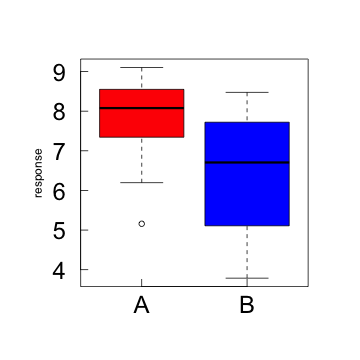
\includegraphics[width=0.4\linewidth]{lectures/day_2_LM_refresh_I/figures/unnamed-chunk-43-1.png}
        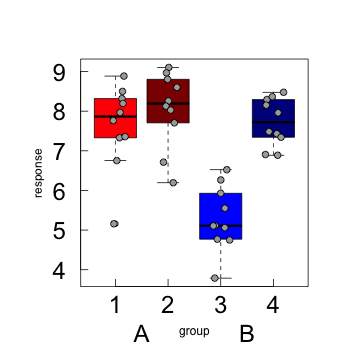
\includegraphics[width=0.4\linewidth]{lectures/day_2_LM_refresh_I/figures/unnamed-chunk-44-1.png}
    \end{figure}
\end{frame}

\begin{frame}
    \frametitle{Residuals with and without the information on grouping}

    \begin{columns}
        \begin{column}{0.5\textwidth}
            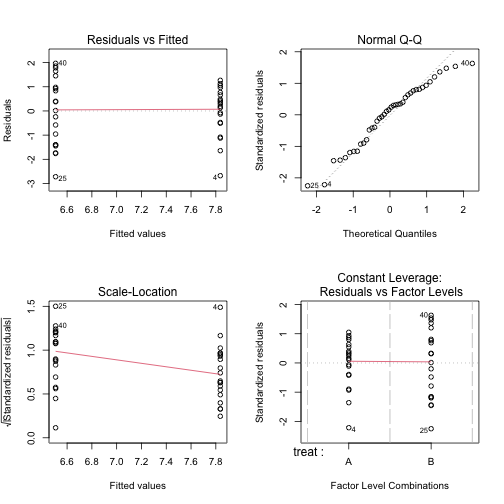
\includegraphics[width=\textwidth]{lectures/day_2_LM_refresh_I/figures/unnamed-chunk-47-1.png}
            \scalebox{0.75}{
                \lstinputlisting[]{lectures/day_2_LM_refresh_I/outputs/output_13_1.txt}
            }
        \end{column}
        \begin{column}{0.5\textwidth}
            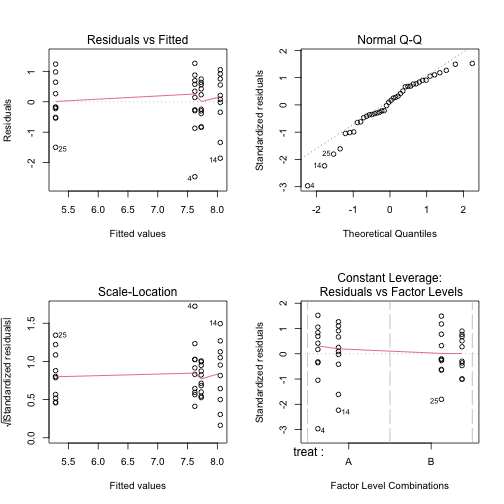
\includegraphics[width=\textwidth]{lectures/day_2_LM_refresh_I/figures/unnamed-chunk-49-1.png}
            \scalebox{0.75}{
                \lstinputlisting[]{lectures/day_2_LM_refresh_I/outputs/output_13_2.txt}
            }
        \end{column}
    \end{columns}
    
\end{frame}

\begin{frame}
    \frametitle{Recapitulation Day 2}
    \textbf{After today you should know and understand:}
    \begin{itemize}
        \item How a \textbf{linear model} is expressed as a formula, in matrix notation, and in R code.
        \item What the \textbf{off-diagonals} in an error covariance matrix are.
        \item The \textbf{assumptions} of linear models.
        \item How linear models are fitted using \textbf{maximum likelihood}.
        \item How a linear model is implemented, diagnosed, and interpreted in R.
        \item The terms \textbf{model coefficient}, \textbf{model parameter}, \textbf{residuals}, \textbf{design matrix}, etc., should be clear.
    \end{itemize}
    \vspace{1cm}
    \textbf{This afternoon: Practical exercises about Linear Models in R.}
\end{frame}

\end{document}
